\section{Harnessing Wind Energy}
\label{sec:harnessing_wind}

As has become apparent in section \ref{sec:climate_policy}, there is a significant
need to reduce the carbon emissions from the energy sector. One of the ways to
achieve this is to substitute fossil fuels as an energy source for renewable
sources of energy. While sun and wind power are thought to be the ones most likely
to grow the fastest in the next decades, this section will focus on wind power
and how it can be harnessed. 

\subsection{Extracting Power from the Wind}
\label{sec:extracting_power_from_wind}

The main idea about wind power is that, by using a device (wind turbine) we are 
able to extract energy from the wind (kinetic energy) and transform it into some
other form of energy that is more useful to us (electrical power).\\

Let's consider a model in which air is an incompressible fluid (poor assumption),
with density $\rho$
the unperturbed wind is initially travelling with speed $V_1$ and swept cross-sectional
area $S_1$ and after passing through the wind turbine it is travelling with speed
$V_2$ and swept cross-sectional area $S_2$. See Figure \ref{fig:wind_turbine_model}.

\begin{figure}[ht]
    \centering
    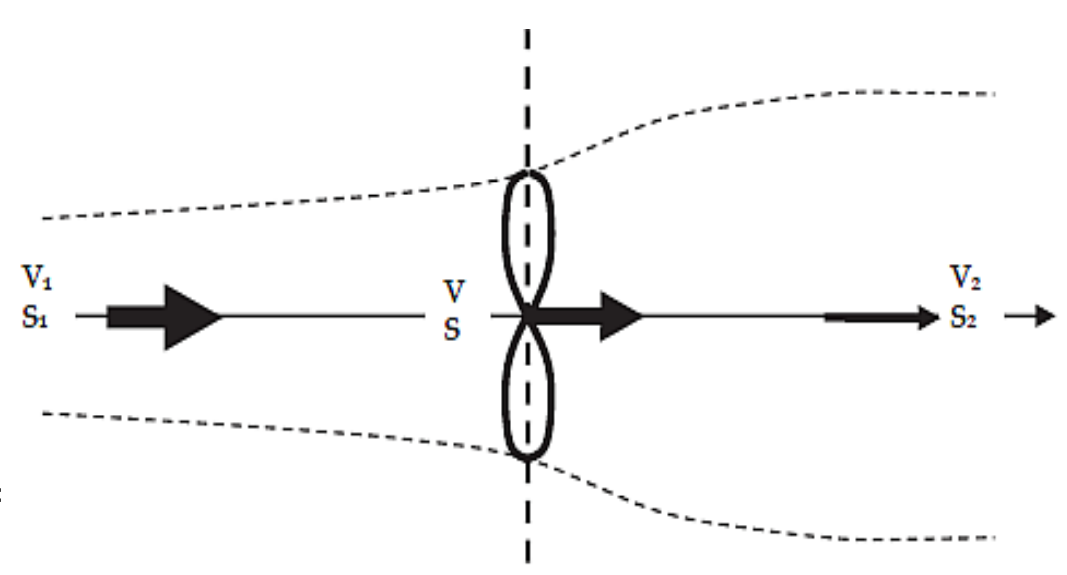
\includegraphics[width=0.65\textwidth]{figures/wind_turbine_model.png}
    \caption{Wind Turbine Model}
    \label{fig:wind_turbine_model}
\end{figure}

\noindent With this in mind we can note a few things. Firstly, the fact that the
turbine extracts kinetic energy suggests that $V_2 < V_1$. Secondly, as per conservation
of mass flow, we can write that
$$
\frac{dm}{dt} = \rho V_1 S_1 = \rho V_2 S_2 = \rho SV = \text{constant}
$$
and from it we can derive the power we are able to extract from the wind:
\begin{align*}
    \text{Force applied by wind} \quad & F = m \frac{dV}{dt} = \frac{dm}{dt} \Delta V
    = \rho SV (V_1 - V_2) \\
    \text{Power from wind} \quad & P = F \frac{dx}{dt} = \rho SV^2(V_1 - V_2)
\end{align*}

Similarly, we can write the power in terms of change of kinetic energy:
$$
P = \frac{1}{2} \frac{dm}{dt} (V_1^2 - V_2^2) = \frac{1}{2} \rho SV (V_1^2 - V_2^2)
$$
and equating the two expressions for power we get:
\begin{align*}
    \frac{1}{2} \rho SV (V_1^2 - V_2^2) &= \rho SV^2(V_1 - V_2) \\
    \frac{1}{2} (V_1 + V_2)\cancel{(V_1 - V_2)} &= V \cancel{(V_1 - V_2)}
\end{align*}
\begin{gather*}
    V = \frac{1}{2}(V_1 + V_2)\\
    \boxed{P = \frac{1}{4} \rho S(V_1^2 - V_2^2)(V_1 + V_2)}
\end{gather*}
so we have obtained a formula for the total available power to be extracted from
the wind.\\

It is evident however, that due to limtiations similar to those we encountered
in Carnot cycles in thermodynamics we will not be able to harness 100\% of all
available power. It therefore follows that we will be interested in how efficient
our wind turbine is, and therefore can define the \textbf{performance coefficient}
$C_p$. To do that we firstly introduce the concept of the kinetic power content, 
$W$ i.e. the power contained in a unit mass of air moving with initial speed $V_1$:
$$
W = \frac{1}{2}\frac{dm}{dt} V_1^2 = \frac{1}{2} \rho SV_1^3
$$
and so we define the performance coefficient as the power extracted from the wind
turbine divided by the kinetic power the wind had in the first place:
$$
C_p = \frac{P}{W} = \frac{\cancelto{\frac{1}{2}}{\frac{1}{4}\rho S}(V_1^2 - V_2^2)(V_1 + V_2)}
{\cancel{\frac{1}{2} \rho S}V_1^3} = \frac{(V_1^2 - V_2^2)(V_1 + V_2)}{2V_1^3}
$$
to which we can introduce the interference factor $b=V_2/V_1$ and make some 
substitutions:
\begin{align*}
    P &= \frac{1}{4} \rho S V_1^3 (1 - b^2)(1 + b) \\
    C_p &= \frac{1}{2}(1 - b^2)(1 + b)
\end{align*}
and finally we can plot the performance coefficient as a function of the interference
factor (see figure \ref{fig:performance_coefficient}).
\begin{figure}[h]   
    \centering
    \begin{tikzpicture}

        \begin{axis}[
            axis lines = left,
            xlabel = $b$,
            ylabel = {$C_p$},
            xmin=0, xmax=1,
            ymin=0, ymax=0.6,
            xtick={0,0.333, 0.5,1},
            ytick={0,0.2,0.4,0.6},
        ]
        \addplot [
            domain=0:1, 
            samples=100, 
            color=red,
        ]
        {0.5*(1-x^2)*(1+x)};
        % Vertical line at b=1/3 to show maximum point
        \addplot[black, thick, dotted] coordinates {(0.333, 0) (0.333, 0.593)};

        \end{axis}
    \end{tikzpicture}
    \caption{Performance coefficient as a function of interference factor}
    \label{fig:performance_coefficient}
\end{figure}

\noindent From the plot we can see that the maximum performance coefficient is
$C_p = 0.593$ and it occurs at $b=1/3$. This is the \textbf{Betz Limit} and it
is the maximum theoretical power fraction that can be extracted from a wind stream.
Analytically we can write:
$$
\frac{dC_p}{db} = \frac{1}{2} (1 - 3b)(1+b) \quad \implies \quad b = \frac{1}{3}
\quad \therefore V_2 = \frac{1}{3}V_1
$$
which using the above definition for $P$ we get:
$$
P = \frac{16}{27} \frac{\rho}{2} V_1^3 S
$$
and assuming a circular swept area of diameter $D$ i.e. $S = \pi D^2/4$ we get:
$$
P = \frac{16}{27} \frac{\rho}{2} V_1^3 \frac{\pi D^2}{4}
$$

\noindent In reality, just like with the Carnot cycle, it is not realistic to obtain this
maximum efficiency due to frictional losses in the rotor, drag due to blade surface
roughness and other mechanical imperfections. In practice, the maximum efficiency
is around 40-45\%.

\subsection{Wind-Speed Distributions}
\label{sec:windspeed_distributions}

In order to be able to estimate how much power will be able to be extracted from
the wind it is important to know the wind speed distribution as to place wind 
turbines in the most optimal of places.\\

We typically approximate the wind-speed distribution $f(V)$ as a Rayleigh distribution:
$$
f(V)_{\text{Rayleigh}} = \frac{V}{c^2} e^{-(V/c)^2} \quad \quad 0 \leq V < \infty
$$
and in some situations, the Weibull distrubution might be more appropriate:
$$
f(V)_{\text{Weibull}} = \frac{k}{c} \left(\frac{V}{c}\right)^{k-1} e^{-(V/c)^k}
\quad \quad 0 \leq V < \infty
$$
where $c$ and $k$ are distribution parameters. The Weibull goes to a Rayleigh
when $k=2$.\\

We can therefore use the Rayleigh distribution to estimate the average extractable
power. For a turbine operating in a flow of instantaneous speed $V$ the extractable 
power $P$ is:
$$
P = C_p \frac{V^2}{2} \frac{dm}{dt} = \frac{1}{2} C_p \rho S V^3
$$
and as per what we said before, we can find a mean for the power by using the mean
of the distribution of wind speeds:
\begin{align*}
    \overline{P(V)} &= C_p \int_{V_{\text{min}}}^{V_{\text{max}}} P(V) f(V)_{\text{Rayleigh}} dV\\
    &= C_p \int_0^\infty \frac{\rho S V^3}{2} f(V)_{\text{Rayleigh}} dV\\
    &= \frac{C_p \rho S}{2} \int_0^\infty V^3 f(V)_{\text{Rayleigh}} dV\\
    \Aboxed{\overline{P(V)} &= \frac{C_p \rho S}{2} \overline{V^3}}
\end{align*}

Note that $\overline{V^3}$ is not the same as $\overline{V}^3$. In this case, we
use $\overline{V^3} = c^3 3\sqrt{\pi}/4$ for the equations above.\\

It therefore follows that at the Beltz Limit:
$$
\boxed{
\overline{P(V)}_{\text{max}} = \frac{16}{27} \frac{\rho}{2} \frac{\pi D^2}{4}
\frac{6}{\pi} \overline{V}^3 = \rho \left( \frac{2}{3} D \right)^2 \overline{V^3}}
$$

Another factor to bear in mind is the fact that the wind speed is not constant
on the vertical axis: it increases with height. This is in fact the reason why
wind turbines have been getting taller and larger in diameter over the years.

A good model for the vertical distribution of speeds is a logarithmic profile 
as follows:
$$
\boxed{V(z) = k \ln \left(\frac{z}{z_0}\right)}
$$
where $k$ is a constant and $z_0$ is the \textbf{roughness length} - a measure
of the height above the surface at which the windspeed theoretically becomes zero.
Roughness length is indeed determined by the roughness of ther surface, i.e. how
much of an impediment does it pose to the wind travelling above it.

\begin{table}[h]
    \centering
    \begin{tabular}{c|c}
        \textbf{Surface} & \textbf{Roughness Length (m)}\\
        \hline
        Sand & 0.0001-0.001\\
        Open Sea & 0.005\\
        Grass & 0.01-0.1\\
        Suburban & 0.2-0.4\\
        Urban & 0.35-0.8\\
        Forest & 0.9-1\\
    \end{tabular}
    \caption{Roughness Lengths}
    \label{tab:roughness_lengths}
\end{table}

\subsection{Issues with Wind Power}
\label{sec:issues_with_wind_power}

There are a number of issues with wind power that have to be considered. Here is
a non-exhaustive list:
\begin{itemize}
    \item Wind supply is not constant, meaning that there will be times when generation
    is needed but is not able to be provided, and times of excess generation. This
    has to be addressed by having a backup power source, or by having a way to store
    the excess energy.
    \item They are noisy and can be an eyesore. 
    \item Power transmission/distribution is an issue. Wind farms are typically
    located in remote areas, meaning that the power has to be transmitted over long
    distances, leading to potential losses.
    \item There is a non-zero carbon impact of buliding and replacement of wind
    turbines. An average lifespan for a wind turbine is 10-20 years.
    \item Large scale deployment of wind turbines create wake effects, i.e. the
    performance of a turbine is affected when it is behind another one. Turbine 
    separation must be 5-10x rotor diameter.
\end{itemize}

% Section glossary


